\section{Схемотехнический анализ радиоэлектронного средства}

% Рассказывается про то как функционирует устройство, на основании того
% как объяснено функционирование принципиальной схемы, взятой из
% журнала. Приведен расчёт электрических параметров потенциометров и
% транзистора из схемы. Расчёт именно этих параметров обоснован тем, что
% они будут необходимы в дальнейшем для расчёта выделяемой теплоты.
% Возможно, будет использован САПР SimulIDE вместо расчёта
% схемы в ручную.

\subsection{Описание принципа работы
  проектируемого радиоэлектронного средства.}

Поскольку статья о тестовом сервотестере написана в иностранном
журнале, схема электрическая принципиальная в нём выполнена не по
отечественному ГОСТ.

\begin{figure}[H]
  \centering
  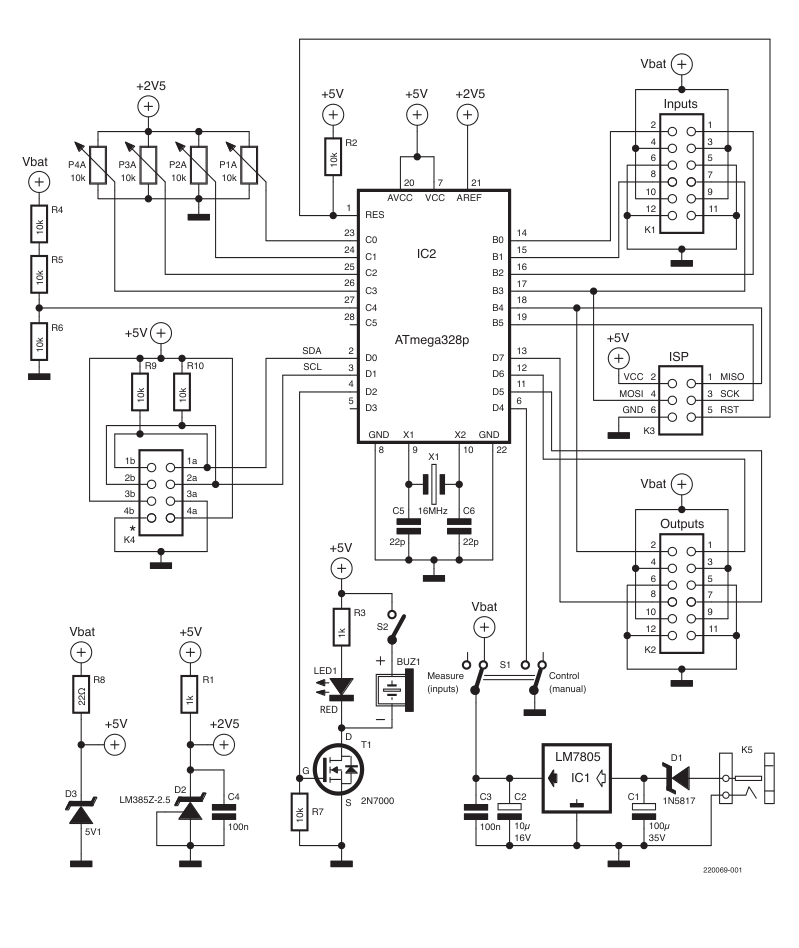
\includegraphics[scale = 0.50]{SchematicsShotFromElector.png}
  \caption{Электрическая принципиальная схема устройства}
\end{figure}

На приложенной схеме в центре видно микроконтроллер подключенный к
кристаллу с частотой колебаний 16 МГц, который в свою очередь
подключен к конденсаторам C5 и С6. Четыре ножки GPIO — PB0-PB3
подключены к разъёму K1. Выводы для серво сигнала — PD5, PD6, PD7 и
PB4 подключены к разъёму K2. Два этих разъёма разведены таким
образом, что к ним можно подключить стандартный для сервопривода
кабель ~\cite{Elector521}.

Четыре потенциометра подключены к аналоговым входам микроконтроллера
PC0-PC3. Питание подключается через делитель напряжения из резисторов
R4-R6 к аналоговому входу PC4. Отношение между суммой сопротивлений
R4, R5 и сопротивлением R6 должно быть 2 к 1 соответственно, но их
абсолютные значения не критичны. Использование трёх резисторов одного
значения облегчает их сортировку для точности ~\cite{Elector521}.

Для того чтобы измерять напряжение источника питания нужен
аналоговоцифровой преобразователь и опорное напряжение не относящиеся
к самому напряжению питания.  В микроконтроллере уже есть опорное
напряжение в 1,1 Вольт, однако это значение несколько мало. И поэтому
используется источник опорного напряжения LM385-2.5 обозначенный как
D2, как внешнее опорное напряжение в 2,5 Вольта. Этот элемент более
точен, чем простой двух контактный зенеровский диод
~\cite{Elector521}.

К коннектору K4 подключается OLED дисплей по типу SSD1306.  У
дисплея должен быть порт I2C, но он будет подключаться к
порту I2C микроконтроллера, но к компонентам PD0 и PD1. Шина
I2C эмулируется программным обеспечением. Так выходит из-за
того, что шина I2C на данном микроконтроллере находится на
том же пине, что и аналоговый вход PC4, который уже используется для
измерения напряжения питания ~\cite{Elector521}.

Резисторы R9 и R10 это подтягивающие резисторы для шины I2C.

Ползунковый переключатель S1 типа DPDT1 используется для
выбора режима работы сервотестера. В ручном режиме переключатель
соединяет напряжения питания номиналом 5 Вольт и коннекторы
сервоприводов. В режиме ввода он предотвращает неправильное включение
напряжений ~\cite{Elector521}.

Сама по себе схема достаточно проста,состоит из небольшого числа
компонентов, но тем не менее может работать в нескольких режимах и
схемах включения, что выглядит как положительные черты относительно
того в каких вариантах использования оказывается устройство.

\subsection{Расчет электрических параметров 
  и режимов работы 
  отдельных каскадов проектируемого устройства}

% Виктор Сильвестрович сказал здесь вставить расчет куска схемы с пищалкой

Сердцем данной схемы является микроконтроллере устройство.
В случае микроконтроллерных устройств может существовать несколько
способов задачи тактовой частоты, таких как:
\begin{enumerate}
\item Внутренний RC-генератор микроконтроллера;
\item Внешняя RC-цепочка на печатной плате;  
\item Внешний кварцевый резонатор.
\end{enumerate}

В данной схеме устройства для тактирования микроконтроллера
используется внешний кварцевый резонатор. Вместе с двумя
конденсаторами он образует колебательный контур.

Конденсаторы образуют нагрузку колебательного контура, в который
входит кварцевый резонатор, таким образом обеспечивая устойчивый старт
колебаний и генерацию сигнала кварцевого резонатора именно на первой
гармонике. На профессиональном жаргоне эти конденсаторы называют
нагрузочными.
% https://electronix.ru/forum/topic/13466-zachem-nuzhny-kondery-u-kvartsevogo-rezonatora-v-mk/#comment-92140

Для работоспособности микроконтроллерного устройства важно рассчитать
необходимые номиналы нагрузочных конденсаторов. Это можно сделать по
формуле, согласно документации производителя микроконтроллерного
устройства ~\cite{microchip-Calculating-crystal-load-capacitor}.
% https://microchip.my.site.com/s/article/Calculating-crystal-load-capacitor

\begin{equation}
  C_L = \frac{(C_1 \cdot C_2 )}{C_1 + C_2 + C_{stray}}
\end{equation}
Где,
$C_L$ - нагрузочная ёмкость, указанная в документации производителя микроконтроллерного устройства;
$С_1$ и $C_2$ - ёмкость первого и второго нагрузочного конденсатора соответственно;
$C_{stray}$ - паразитная ёмкость, возникающая из-за пинов чипа
микроконтроллерного устройства и паразитных ёмкостей печатной платы и
дорожек. Обычно аппроксимируется равным 5 пикофарад ~\cite{microchip-Calculating-crystal-load-capacitor}.

Если принять что значения ёмкости конденсаторов $C_1$ и $C_2$ равны,
то исходную формулу можно переписать, как:
\begin{equation}
  С_1 = С_2 = 2 \cdot (C_L - C_{stray})
\end{equation}


Согласно документации производителя микроконтроллерного устройства,
рекомендованное значение $С_1$ и $С_2$ для микроконтроллерного
устройства Microchip ATMega328P находится в пределах от 12 до
22 пикофарад ~\cite{microchip-atmega328p-datasheet}.

Согласно документации производителя тактирующего кварцевого резонатора, значение $С_L$ 
равно 20 пикофарад ~\cite{crystal-datasheet}.

% Таким образом ёмкость конденстаторов можно расчитать, как:
% $$C_1 = C_2 = 2 \cdot (20 - 5) = 30 пф$$

% Однако данное значение в 30 пикофаррад не сходятся с выбранными на
% схеме емкостями в 22 пикофаррада. Возможно, что это значение
% получилось в результате неправильно выбранного значения для паразитной
% ёмкости $C_{stray}$.

Зная ёмкость конденсаторов из схемы и нагрузочную ёмкость из
документации производителя тактирующего кристалла, можно
рассчитать паразитную ёмкость, в пределах значений которой должна
оказаться ёмкость дорожки на печатной платы и ножек чипа
микроконтроллерного устройства. Сделать это можно по формуле:

\begin{equation}
  C_{stray} = C_L - \frac{C_1}{2}
\end{equation}

Таким образом:
$$C_{stray} = 20 - \frac{22}{2} = 20 - 11 = 9пф$$

Наличие известных приделов паразитной ёмкости, облегчит разработку
изделия на этапе проектирования и расчёт электромагнитной
совместимости печатной платы.

\newpage

%%% Local Variables:
%%% mode: LaTeX
%%% TeX-master: "main"
%%% End:
